\begin{frame}{Experimental Setup}

    \begin{block}{Experimental testbed}
        Experiments presented in this paper were carried out using the Grid'5000 testbed, supported by a scientific interest group hosted by Inria and including CNRS, RENATER and several Universities as well as other organizations (see https://www.grid5000.fr).
    \end{block}
    
    \begin{block}{Hardware and budget allocated}
        One evaluation on chuc cluster, using 4*A100 40G of VRAM GPU, is taking around 40 minutes. Each algorithms have a budget of 50 evaluations, including the 10 sampling evaluation of BO. 
    \end{block}


    
    
\end{frame}
%---------------------------------- Sampling experiment -------------------------------
\begin{frame}{Sampling experiment : Latin Hypercube Sampling}
    
    \begin{columns}
        \begin{column}{0.4\textwidth}
            
            Objective : Explore the space and define a lower bound for next experiments

            \begin{figure}
                \centering

                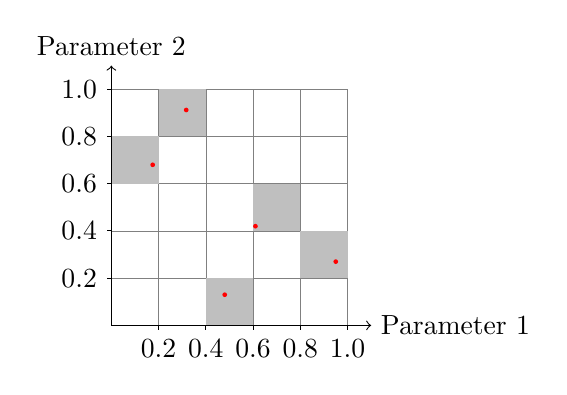
\begin{tikzpicture}[scale=3]

    % Define the grid
    \draw[step=0.2,gray,very thin] (0,0) grid (1,1);
    
    % Shade specific squares
    \fill[gray!50] (0.0,0.6) rectangle (0.2,0.8);
    \fill[gray!50] (0.2,0.8) rectangle (0.4,1.0);
    \fill[gray!50] (0.4,0.0) rectangle (0.6,0.2);
    \fill[gray!50] (0.6,0.4) rectangle (0.8,0.6);
    \fill[gray!50] (0.8,0.2) rectangle (1.0,0.4);
    
    % Draw red points
    \fill[red] (0.175,0.68) circle (0.01);  % Point in the first square
    \fill[red] (0.317,0.912) circle (0.01);  % Point in the second square
    \fill[red] (0.48,0.13) circle (0.01);  % Point in the third square
    \fill[red] (0.61,0.42) circle (0.01);  % Point in the fourth square
    \fill[red] (0.95,0.27) circle (0.01);  % Point in the fifth square
    
    % Draw the axes
    \draw[->] (0,0) -- (1.1,0) node[right] {Parameter 1};
    \draw[->] (0,0) -- (0,1.1) node[above] {Parameter 2};
    
    % Add ticks and labels
    \foreach \x in {0.2,0.4,0.6,0.8,1.0} {
      \draw (\x,0) -- (\x,-0.02) node[below] {\x};
      \draw (0,\x) -- (-0.02,\x) node[left] {\x};
    }
    
\end{tikzpicture}
                \caption{LHS illustration with $g=5$ samples}
            \end{figure}
            
        \end{column}

        \begin{column}{0.6\textwidth}
            \begin{figure}
                \centering
                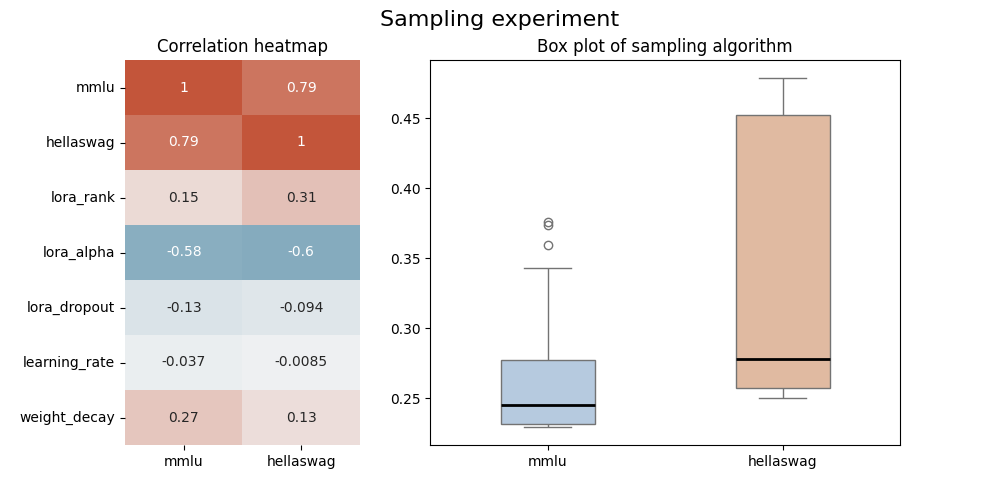
\includegraphics[width = \textwidth]{imgs/experiments/lhs/lhs.png}     
                \caption{Results of LHS Experiment\footnote[5]{ \textit At left : correlation between metrics and hyperparameters // At right : metrics distribution}}         
            \end{figure}
            
        \end{column}
\end{columns}  

\end{frame}



%---------------------------------- Bayesian Optimization -------------------------------
\begin{frame}{Results : Bayesian Optimization} 
    
    \begin{columns}
    
        \begin{column}{0.6\textwidth}
            \begin{block}{Score over time}
                \begin{figure}
                    \centering
                    \begin{tikzpicture}[domain = 0:50,scale = 0.7]
    \tikzstyle{point} = [only marks, mark = triangle*, mark size = 3, opacity = 0.5]
    \begin{axis}[
        legend pos=south east,
        ymin = 0.2,
        x=3.2,
        y =450
    ]
    \addplot [blue,point] table {imgs/experiments/bo/bo_hs.dat};
    \addlegendentry{$f(x)$}

    \draw[color=red, dashed](axis cs:10,0) -- (axis cs:10,0.5);




    \end{axis}
\end{tikzpicture}
                    \caption{Results on validation dataset for BO-GP Algorithm}
                \end{figure}
            
            \end{block}   
        \end{column}

        \begin{column}{0.4\textwidth}
            \begin{block}{Results}
                Hellaswag($D_{val}$) Best score : 47,91\%        
            \end{block}

            \begin{block}{Behavior}

                \begin{itemize}
                    \item Fast convergence after sampling phase
                    \item Few shots emphasing exploration with lower score
                \end{itemize}
                
                
            \end{block}
             
        \end{column}
    \end{columns}    
\end{frame}

%---------------------------------- SOO -------------------------------
\begin{frame}{Results : SOO} 
    
    \begin{columns}
    
        \begin{column}{0.6\textwidth}
            \begin{block}{Score over time}
                \begin{figure}
                    \centering
                    \begin{tikzpicture}[domain = 0:50,scale = 0.7]
    \tikzstyle{point} = [only marks, mark = triangle*, mark size = 3, opacity = 0.5]
    \begin{axis}[
        legend pos=south east,
        ymin = 0.2,
        x=3.2,
        y =450
    ]
    \addplot [red,point] table {imgs/experiments/soo/soo_hs.dat};
    \addlegendentry{$f(x)$}




    \end{axis}
\end{tikzpicture}
                    \caption{Results on validation dataset for SOO Algorithm}
                \end{figure}
            
            \end{block}   
        \end{column}

        \begin{column}{0.4\textwidth}
            \begin{block}{Results}
                Hellaswag($D_{val}$) Best score : 47.84\%        
            \end{block}

            \begin{block}{Behavior}

                \begin{itemize}
                    \item A lot of low score evaluation, due to one hyperparameter
                    \item maximum depth of 8 (only 2 points with depth = 8)
                \end{itemize}

            \end{block}
             
        \end{column}
    \end{columns}    
\end{frame}


%---------------------------------- BaMSOO -------------------------------
\begin{frame}{Results : BaMSOO} 
    
    \begin{columns}
    
        \begin{column}{0.6\textwidth}
            \begin{block}{Score over time}
                \begin{figure}
                    \centering
                    \begin{tikzpicture}[domain = 0:50,scale = 0.7]
    \tikzstyle{point} = [only marks, mark = triangle*, mark size = 3, opacity = 0.5]
    \begin{axis}[
        legend pos=south east,
        ymin = 0.2,
        x=3.2,
        y =450
    ]
    \addplot [purple,point] table {imgs/experiments/bamsoo/bamsoo_hs.dat};
    \addlegendentry{$f(x)$}




    \end{axis}
\end{tikzpicture}
                    \caption{Results on validation dataset for BaMSOO Algorithm}
                \end{figure}
            
            \end{block}   
        \end{column}

        \begin{column}{0.4\textwidth}
            \begin{block}{Results}
                Hellaswag($D_{val}$) Best score : 47.84\% \\
                Do not achieve to overperform SOO best score   
            \end{block}

            \begin{block}{Behavior}

                \begin{itemize}
                    \item Prevent SOO unpromising evaluation (16 approximated evaluations)
                    \item maximum depth of 8 (8 points with depth = 8)
                \end{itemize}

            \end{block}
             
        \end{column}
    \end{columns}    
\end{frame}



%%%%%%%%%%%%%%% COMPARISON %%%%%%%%%%%%%%
\begin{frame}{Comparison and analysis}

    \begin{columns}
    
        \begin{column}{0.45\textwidth}

            \begin{block}{Analysis}
                \begin{itemize}
                    \item Upper Bound on Hellaswag is irrelevant
                    \item Only BO-GP beat LHS 
                    \item with more high-performing solution, BaMSOO overperform SOO on MMLU
                \end{itemize}
                
            \end{block}\vspace*{-10pt}
            
            \begin{block}{Results}
                \begin{table}[h!]
    \centering
    \begin{tabular}{|c||c|c|}
    \hline
       & Hellaswag & MMLU\\
    \hline\hline
       Lower Bnd$^1$  & 47.90 & 37.61 \\
       Upper Bnd$^2$  & \textit{41.5} & 49.3 \\
    \hline
       BO-GP  & \textbf{47.91} & \textbf{38.11} \\
       SOO  & 47.84 & 37.42 \\
       BaMSOO  & 47.84 & 37.50 \\
    \hline
    \end{tabular}
    \caption{Bound and best score for datasets (val and test)}
\end{table} 
\vspace*{-15pt}{\footnotesize 1 : LHS results; 2 : Meta Fine tuning }
            \end{block}
            
            
            
        \end{column}

        \begin{column}{0.45\textwidth}
            \begin{block}{Score over time on testing dataset}
                \begin{figure}
                    \centering
                    \begin{tikzpicture}[domain = 0:50,scale = 0.7]
    \tikzstyle{point} = [only marks, mark = triangle*, mark size = 3, opacity = 0.5]
    \begin{axis}[
        legend pos=south east,
        ymin = 0.2,
        x=3.2,
        y =700
    ]
    \addplot [blue,point, visible on = <1> ] table {assets/tikz_picture/global_results/bo_mmlu.dat};
    \addlegendentry{BO}

    \addplot [red, point, visible on = <2>] table {assets/tikz_picture/global_results/soo_mmlu.dat};
    \addlegendentry{SOO}

    \addplot [violet, point, visible on = <3>] table {assets/tikz_picture/global_results/bamsoo_mmlu.dat};
    \addlegendentry{BaMSOO}



    \addplot [blue,point, visible on = <4>] table {assets/tikz_picture/global_results/bo_mmlu.dat};
    \addplot [red, point, visible on = <4>] table {assets/tikz_picture/global_results/soo_mmlu.dat};
    \addplot [violet, point, visible on = <4>] table {assets/tikz_picture/global_results/bamsoo_mmlu.dat};




    \end{axis}
\end{tikzpicture}
                    \caption{Results on testing dataset for the three algorithms}
                \end{figure}
            
            \end{block}  
             
        \end{column}
    \end{columns}    

\end{frame}